This section describes the interconnected components in a water distributed network (WDN) using Graph Theory. We investigate three different graph networks; a simplified graph model not including pump and valve edges, one which includes pump and valve edges, and one which describes the implemented laboratory network.


\subsection{Basic Graph Theory}

A \textbf{directed graph} is a set of nodes $ \{v_1,..,v_n\} $ and a set of edges $ \{e_1,..,e_m\} $, with each edge associated with a node pair $ \{v_i,v_j\} $ and an arrow pointing from $ v_i $ to $ v_j $. \\

The \textbf{Incidence Matrix} $H$ of a directed graph is defined as:
\begin{equation*}
	H_{i,j} = \begin{cases}
		1 & \text{If the $j$th edge s leaving the $i$th node}\\
		-1 & \text{If the $j$th edge enters the $i$th node} \\
		0 & \text{If the $j$th edge is unconnected to the $i$th node} 
		
	\end{cases}\\
\end{equation*} 
\begin{equation*}
	H\in \mathbb{R}^{n\times m}
\end{equation*}
With $n$ and $m$ being the number of nodes and edges respectively.

The \textbf{Reduced Incidence Matrix $\bar{H}$} is obtained by choosing one of the nodes as reference and removing the corresponding row from $ H $.

\begin{equation*}
	\bar{H}\in \mathbb{R}^{n-1\times m}
\end{equation*}

The \textbf{spanning tree} is the connected graph but with no loops, i.e you cannot find a route around the graph where you start and end in the same node without entering a node more than once. 

A \textbf{chord} is an edge which creates exactly one loop if added to the spanning tree. 

A \textbf{loop} is a unique route along the edges of the graph, where all nodes are unique except the end node. In a loop the end node must also be the start node. 

The \textbf{loop matrix} $B$ is defined as:
\begin{equation*}
	B_{i,j} = \begin{cases}
		1 & \text{If the direction of the $ i $th loop and the} \text{ $j$th edge agree}\\
		-1 & \text{If the direction of the $ i $th loop and the} \text{ $j$th edge do not agree}\\
		0 & \text{If the $ i $th loop does not include the $ j $th edge}\\
	\end{cases}
\end{equation*}

But can also be calculated as shown below:

\begin{equation}\label{eq:LoopMatrix}
	B = \begin{bmatrix}
		I & -\bar{H}_{C}^{T}\cdot\bar{H}_{T}^{-T}
	\end{bmatrix}
\end{equation}

With $\bar{H}_{C}$ being the matrix containing only chord columns of the reduced incidence matrix. Similarly, $\bar{H}_{T}$ contains only the non-chord columns. 

\begin{equation*}
	B\in \mathbb{R}^{c\times m}
\end{equation*}

With $c$ and $m$ being the number of chords and edges respectively.

\newpage
\subsection{Simplified System}
The graph network shown in \cref{fig:graph} is a simplified graph network of the WDN laboratory implementation and has mainly been used to confirm basic graph theoretical concepts. This model does not include pump and valve edges.  

\begin{figure}[h!]
	\centering
	\includegraphics[width=0.4\textwidth]{Pictures/Graph.png}
	\caption{Graph of simplified WDN network \cite{Rathore930}}
	\label{fig:graph}
\end{figure}

When applying the rules shown above for the simplified graph model of the WDN the incidence matrix becomes:

\begin{equation}
	H = \begin{bmatrix}
		1 & 0 & 1 & 0 & 0 & 0 & 0\\
		-1 & 1 & 0 & 0 & 0 & 0 & 0\\
		0 & 0 & -1 & 1 & 1 & 0 & 0\\
		0 & -1 & 0 & -1 & 0 & 1 & 0\\
		0 & 0 & 0 & 0 & -1 &  0  & -1\\
		0 & 0 & 0 & 0 & 0 & -1 & 1
	\end{bmatrix}
	\label{eq:H_simplified}
\end{equation} 


The reduced incidence matrix is formed by taking an arbitrary node as a reference, and removing the corresponding row from \cref{eq:H_simplified}. We chose the $4$th node, which results in the following reduced incidence matrix:

\begin{equation}
	\bar{H} = \begin{bmatrix}
	1 & 0 & 1 & 0 & 0 & 0 & 0\\
	-1 & 1 & 0 & 0 & 0 & 0 & 0\\
	0 & 0 & -1 & 1 & 1 & 0 & 0\\
	0 & -1 & 0 & -1 & 0 & 1 & 0\\
	0 & 0 & 0 & 0 & -1 &  0  & -1
	%0 & 0 & 0 & 0 & 0 & -1 & 1
	\end{bmatrix}
\end{equation}

Chords and edges of the spanning tree are:

\begin{equation} 
	\begin{split}
		E_{C} &= \{e_{1},e_{4}\}   \\ E_{T} &= \{e_2,e_3,e_5,e_6,e_7\}
	\end{split}
\end{equation}


\begin{equation}
	B = \begin{bmatrix}
		1 & 0 & 1 & -1 & -1 & 1 & 1\\
		0 & 1 & 0 & 0 & -1 & 1 & 1\\
	\end{bmatrix}
\end{equation}

\clearpage
\subsection{Detailed System}
The graph network shown in \cref{fig:WDNDetailed} is a more detailed graphical representation of the WDN. This includes edges for pumps $(e_{1},e_{11})$ and valve $(e_{3},e_{9})$. 

\begin{figure}[h!]
	\centering
	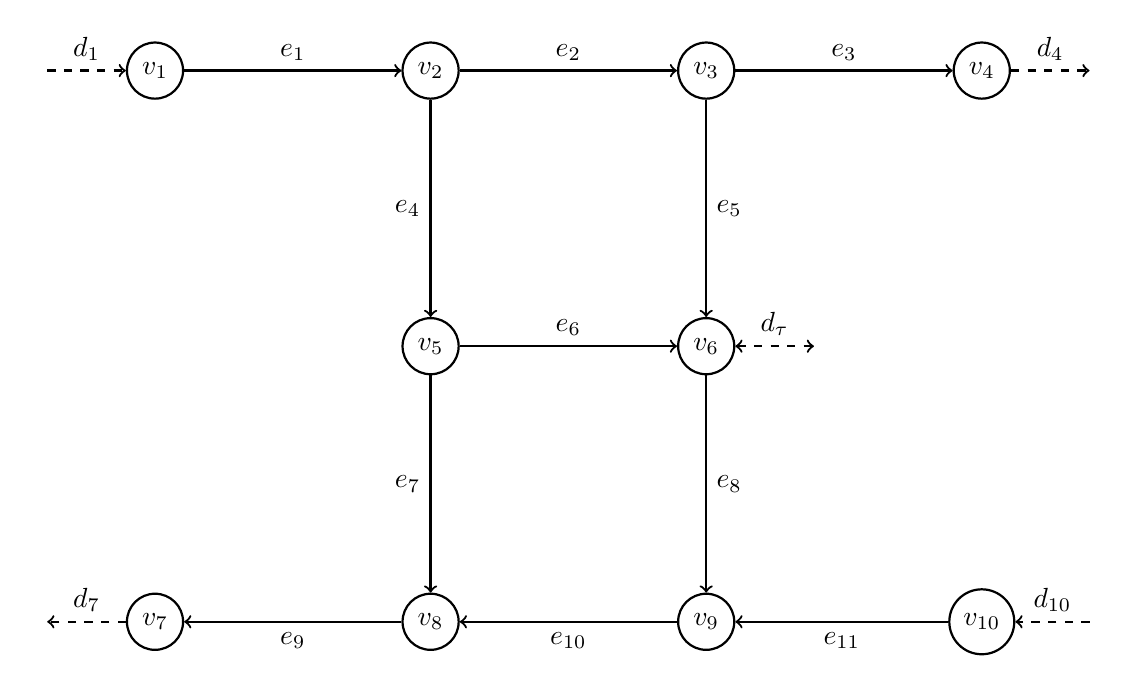
\begin{tikzpicture}[node distance=35mm,thick, main/.style = {draw, circle}] 
		\node (1)  {};
		\node[main] (2) [node distance={15mm},right of=1] {$v_1$}; 
		\node[main] (3) [right of=2] {$v_2$};
		\node[main] (4) [right of=3] {$ v_3 $};
		\node[main] (5) [right of=4] {$ v_4 $};
		\node (6) [node distance={15mm},right of=5] {};
		%Create 2 (3) nodes in middle part of graph
		\node[main] (7) [below of=3] {$ v_5 $};
		\node[main] (8) [below of=4] {$ v_6 $};
		\node (9) [node distance={15mm},right of=8] {};
		%Create 4 (6) nodes in bottom part of the graph
		\node[main] (10) [below of=7] {$v_8$}; 
		\node[main] (11) [left of=10] {$v_7$};
		\node (12) [node distance={15mm},left of=11] {};
		\node[main] (13) [right of=10] {$ v_9 $};
		\node[main] (14) [right of=13] {$ v_{10} $};
		\node (15) [node distance={15mm},right of=14] {};
		
		%Edges with direction
		\path [->] (2) edge node[above] {$e_1$} (3); %Edge v1 -> v2
		\path [->] (3) edge node[above] {$e_2$} (4); %Edge v2 -> v3
		\path [->] (4) edge node[above] {$e_3$} (5); %Edge v3 -> v4
		
		\path [->] (3) edge node[left] {$e_4$} (7); %Edge v2 -> v5
		\path [->] (4) edge node[right] {$e_5$} (8); %Edge v3 -> v6
		\path [->] (7) edge node[above] {$e_6$} (8); %Edge v5 -> v6
		
		\path [->] (7) edge node[left] {$e_7$} (10); %Edge v5 -> v8
		\path [->] (8) edge node[right] {$e_8$} (13); %Edge v6 -> v9
		
		\path [->] (10) edge node[below] {$e_9$} (11); %Edge v8 -> v7
		\path [->] (13) edge node[below] {$e_{10}$} (10); %Edge v9 -> v8
		\path [->] (14) edge node[below] {$e_{11}$} (13); %Edge v10 -> v9
		
		%External flows
		\draw[->,dashed,] (1) -- node[above] {$d_1$} (2); %Create d1
		\draw[->,dashed,] (5) -- node[above] {$d_4$} (6); %Create d4
		\draw[<->,dashed,] (8) -- node[above] {$d_\tau$} (9); %create d_tau
		\draw[->,dashed,] (11) -- node[above] {$d_7$} (12); %create d7
		\draw[->,dashed,] (15) -- node[above] {$d_{10}$} (14); %Create d10
		
	\end{tikzpicture} 
	\caption{Graph network of water distribution network}
	\label{fig:WDNDetailed}
\end{figure}
$ d_1 $ and $ d_{10} $ represent the flow into the system from the pumps.
$ d_4 $ and $ d_7 $ represent the flow out of the system via the valves.
$ d_\tau $ represents the flow in and out of the tank.

The incidence matrix for the graph on \cref{fig:WDNDetailed} is shown below in \cref{eq:H_detailed}.
	
	\begin{equation}\label{eq:H_detailed}
		H = \kbordermatrix{
		& e_1 & e_2 & e_3   & e_4  & e_5 & e_6  & e_7  & e_8  & e_9  & e_{10}  & e_{11}  \\	
		v_1& 1 & 0 & 0   & 0  & 0  & 0  & 0  & 0  & 0  & 0  & 0 \\
		v_2& -1 & 1 & 0  & 1  & 0  & 0  & 0  & 0  & 0  & 0  & 0 \\
		v_3& 0 & -1 & 1  & 0  & 1  & 0  & 0  & 0  & 0  & 0  & 0 \\
		v_4& 0 & 0  & -1 & 0  & 0  & 0  & 0  & 0  & 0  & 0  & 0 \\
		v_5& 0 & 0  & 0  & -1 & 0  & 1  & 1  & 0  & 0  & 0  & 0 \\
		v_6&0 & 0  & 0  & 0  & -1 & -1 & 0  & 1  & 0  & 0  & 0 \\
		v_7& 0 & 0  & 0  & 0  & 0  & 0  & 0  & 0  & -1 & 0  & 0 \\
		v_8& 0 & 0  & 0  & 0  & 0  & 0  & -1 & 0  & 1  & -1 & 0 \\
		v_9& 0 & 0  & 0  & 0  & 0  & 0  & 0  & -1 & 0  & 1  & -1 \\
		v_{10}& 0 & 0  & 0  & 0  & 0  & 0  & 0  & 0  & 0  & 0  & 1 \\
	}
	\end{equation}	
	
The chords and the spanning tree are chosen from \cref{fig:WDNDetailed} \footnote{Note that you can obtain several spanning trees in this network by choosing different edges as chords}
	
\begin{equation*} 
	\begin{split}
		E_{C} &= \{e_{2},e_{6}\}   \\ E_{T} &= \{e_1,e_3,e_4,e_5,e_7, e_8, e_9, e_{10} , e_{11}\}
	\end{split}
\end{equation*}	
	
	By choosing the $10$th node as a reference, and removing it from the incidence matrix, we obtain:
	
	\begin{equation}
		\bar{H} = \kbordermatrix{
		& e_1 & e_2 & e_3   & e_4  & e_5 & e_6  & e_7  & e_8  & e_9  & e_{10}  & e_{11}  \\	
		v_1& 1 & 0 & 0   & 0  & 0  & 0  & 0  & 0  & 0  & 0  & 0 \\
		v_2& -1 & 1 & 0  & 1  & 0  & 0  & 0  & 0  & 0  & 0  & 0 \\
		v_3& 0 & -1 & 1  & 0  & 1  & 0  & 0  & 0  & 0  & 0  & 0 \\
		v_4& 0 & 0  & -1 & 0  & 0  & 0  & 0  & 0  & 0  & 0  & 0 \\
		v_5& 0 & 0  & 0  & -1 & 0  & 1  & 1  & 0  & 0  & 0  & 0 \\
		v_7& 0 & 0  & 0  & 0  & 0  & 0  & 0  & 0  & -1 & 0  & 0 \\
		v_8& 0 & 0  & 0  & 0  & 0  & 0  & -1 & 0  & 1  & -1 & 0 \\
		v_9& 0 & 0  & 0  & 0  & 0  & 0  & 0  & -1 & 0  & 1  & -1 \\
		%v_{10}& 0 & 0  & 0  & 0  & 0  & 0  & 0  & 0  & 0  & 0  & 1 \\
		}
	\end{equation}
	
	\clearpage
	
Furthermore we can define the open-node matrix $F$ and tank matrix $G$:
	
	\begin{equation}\label{eq:ONandTankMatrix}
		F = \kbordermatrix{
			&d_{f_1}&d_{f_2}&d_{f_3}&d_{f_4}\\
		d_1	& 1 & 0 & 0 & 0\\
		d_2	& 0 & 0 & 0 & 0\\
		d_3 & 0 & 0 & 0 & 0\\
		d_4 & 0 & 1 & 0 & 0\\
		d_5 & 0 & 0 & 0 & 0\\
		d_6 & 0 & 0 & 0 & 0\\
		d_7 & 0 & 0 & 1 & 0\\
		d_8 & 0 & 0 & 0 & 0\\
		d_9 & 0 & 0 & 0 & 0\\
		d_{10}& 0 & 0 & 0 & 1 \\
			},
	\qquad
		G = \kbordermatrix{
			&d_{\tau_1}\\
			d_1& 0\\
			d_2& 0\\
			d_3& 0\\
			d_4& 0\\
			d_5& 0\\
			d_6& 1\\
			d_7& 0\\
			d_8& 0\\
			d_9& 0\\
			d_{10}& 0 \\
			}
	\end{equation}

with their reference-respective equivalents given by:

\begin{equation}\label{eq:FbarGbar}
	\bar{F} = F \setminus F_{10\star} \wedge \bar{G} = G \setminus G_{10\star}
\end{equation}

where the notation $X_{10\star}$ denotes the entire 10th row\footnote{Correspondingly, $X_{\star10}$ would denote the entire 10th column} of the matrix $X$ and $\setminus$ is the set relative complement operator. These matrices map demands at their respective nodes into the vector of total demands in the system $d \vee \bar{d}$.

\newpage
\subsection{Implementation of Detailed System}
It is not possible to implement the WDN model shown in \cref{fig:WDNDetailed} in the laboratory due to the fact that we don't have access a $ 4 $-way splitter. Therefore, the graph model is altered to fit a model that can be implemented. The graph is shown in \cref{fig:ImplementedWDN}.
  
\begin{figure}[h!]	
	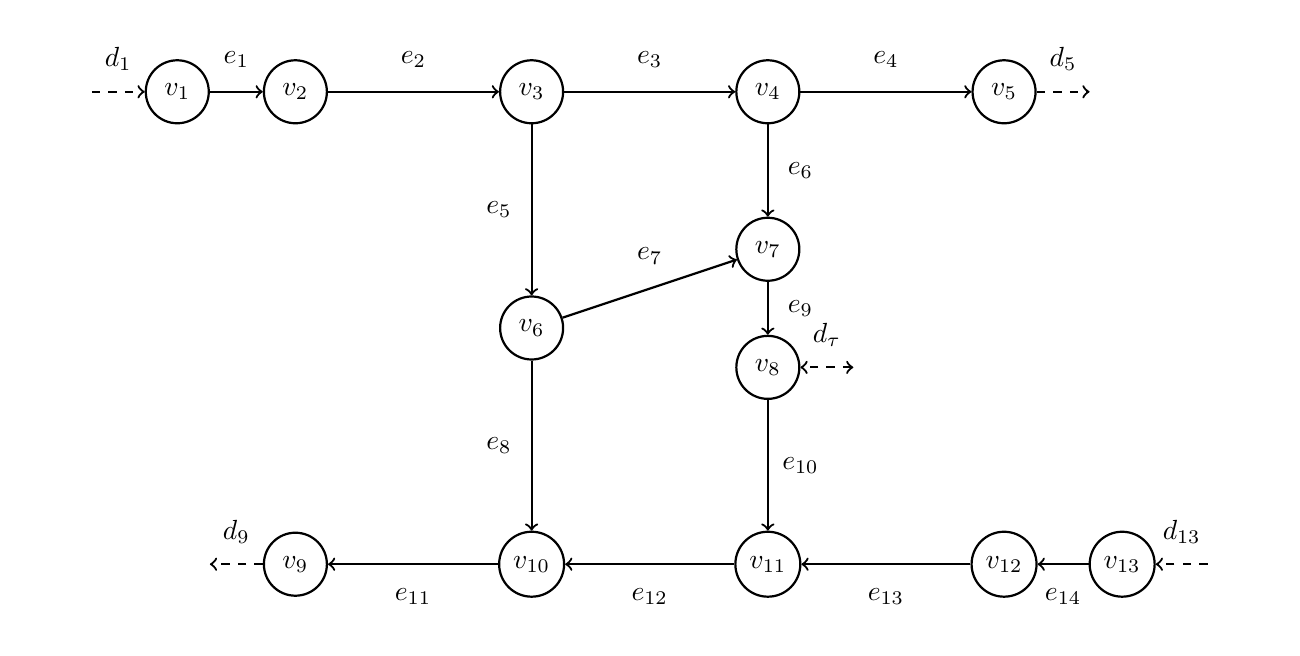
\begin{tikzpicture}[minimum size=0.8cm,node distance=30mm, thick, main/.style = {draw,circle}] 
		\node (1)  {};
		\node[main] (2) [node distance={15mm},right of=1] {$v_1$}; 
		\node[main] (3) [node distance={1.5cm},right of=2] {$v_2$};
		\node[main] (4) [right of=3] {$v_3$};
		\node[main] (5) [right of=4] {$v_4$};
		\node[main] (6) [right of=5] {$v_5$};
		\node (7) [node distance={15mm},right of=6] {};
		%Create 3 (4) nodes in middle part of graph
		\node[main] (8) [below of=4] {$ v_6 $};
		\node[main] (9) [node distance={20mm},below of=5] {$ v_7 $};
		\node[main] (11) [node distance={15mm},below of=9] {$ v_8 $};
		\node (10) [node distance={15mm},right of=11] {};
		%First 5 (7) nodes in bottom part of graph
		\node[main] (12) [below of=8] {$ v_{10} $};
		\node[main] (13) [left of=12] {$ v_9 $};
		\node(14) [node distance={15mm},left of=13] {};
		\node[main] (15) [right of=12] {$ v_{11} $};
		\node[main] (16) [right of=15] {$ v_{12} $};
		\node[main] (17) [node distance={1.5cm},right of=16] {$ v_{13} $};
		\node(18) [node distance={15mm},right of=17] {};
		
		%Edges with direction
		\path [->] (2) edge node[above] {$e_{1}$} (3); 	%Edge v1 -> v2
		\path [->] (3) edge node[above] {$e_{2}$} (4); 	%Edge v2 -> v3
		\path [->] (4) edge node[above] {$e_{3}$} (5); 	%Edge v3 -> v4
		\path [->] (5) edge node[above] {$e_{4}$} (6); 	%Edge v4 -> v5
		
		\path [->] (4) edge node[left] {$e_{5}$} (8); 	%Edge v3 -> v6
		\path [->] (5) edge node[right] {$e_{6}$} (9); 	%Edge v4 -> v7
		\path [->] (8) edge node[above] {$e_{7}$} (9); 	%Edge v6 -> v7
		\path [->] (8) edge node[left] {$e_{8}$} (12); 	%Edge v6 -> v10
		\path [->] (9) edge node[right] {$e_{9}$} (11); 	%Edge v7 -> v8
		\path [->] (11) edge node[right] {$e_{10}$} (15);	 %Edge v8 -> v11
		
		
		\path [->] (12) edge node[below] {$e_{11}$} (13); %Edge v10 -> v9
		\path [->] (15) edge node[below] {$e_{12}$} (12); %Edge v11 -> v10
		\path [->] (16) edge node[below] {$e_{13}$} (15); %Edge v12 -> v11
		\path [->] (17) edge node[below] {$e_{14}$} (16); %Edge v13 -> v12
		
		%External flows
		\draw[->,dashed,] (1) -- node[above] {$d_1$} (2); %Create d1
		\draw[->,dashed,] (6) -- node[above] {$d_5$} (7); %Create d5
		\draw[->,dashed,] (13) -- node[above] {$d_9$} (14); %Create d13
		\draw[->,dashed,] (18) -- node[above] {$d_{13}$} (17); %Create d13
		\draw[<->,dashed,] (10) -- node[above] {$d_\tau$} (11); %Create d_tau
	\end{tikzpicture} 
	\caption{Graph network of implemented water distribution network.}
	\label{fig:ImplementedWDN}
\end{figure}

The incidence matrix becomes:

	\begin{equation}\label{eq:H_detailed_lab}
	H = \kbordermatrix{
		&e_1&e_2&e_3&e_4&e_5&e_6&e_7&e_8&e_9&e_{10}&e_{11}&e_{12}&e_{13}&e_{14} \\	
v_{1}&	1	&0	& 0 & 0 & 0	& 0 & 0	& 0	& 0	& 0 & 0	& 0	& 0	& 0 \\
v_{2}&	-1	& 1 & 0	& 0	& 0	& 0	& 0	& 0	& 0	& 0 & 0	& 0	& 0 & 0 \\
v_{3}&	0	& -1& 1	& 0 & 1 & 0 & 0 & 0 & 0 & 0 & 0	& 0 & 0 & 0 \\
v_{4}&	0	& 0 &-1 & 1 & 0 & 1 & 0 & 0 & 0	& 0	& 0	& 0	& 0	& 0 \\
v_{5}&	0	& 0 & 0	& -1& 0	& 0	& 0	& 0	& 0	& 0	& 0	& 0	& 0	& 0 \\
v_{6}&	0	& 0	& 0	& 0	& -1& 0	& 1	& 1	& 0	& 0 & 0	& 0	& 0 & 0 \\
v_{7}&	0	& 0	& 0	& 0	& 0 & -1& -1& 0	& 1 & 0 & 0	& 0	& 0	& 0 \\
v_{8}&	0	& 0	& 0	& 0	& 0 & 0 & 0 & 0	& -1& 1 & 0	& 0	& 0	& 0 \\
v_{9}&	0	& 0	& 0	& 0	& 0 & 0 & 0 & 0	& 0 & 0 & -1& 0	& 0	& 0 \\
v_{10}&	0	& 0	& 0	& 0	& 0 & 0 & 0 & -1& 0 & 0 & 1 & -1& 0	& 0 \\
v_{11}&	0	& 0	& 0	& 0	& 0 & 0 & 0 & 0 & 0 & -1& 0 & 1 & -1& 0 \\
v_{12}&	0	& 0	& 0	& 0	& 0 & 0	& 0 & 0 & 0 & 0 & 0 & 0 & 1	& -1\\
v_{13}&	0	& 0	& 0	& 0	& 0 & 0	& 0 & 0 & 0 & 0 & 0 & 0 & 0	& 1    
	} 
\end{equation}	


The reduced incidence matrix $ \bar{H} $ for the system given by \cref{eq:H_detailed_lab} is obtained by choosing the node 13 as reference:

	\begin{equation}\label{eq:Hbar_detailed_imp}
	\bar{H} = \kbordermatrix{
		&e_1&e_2&e_3&e_4&e_5&e_6&e_7&e_8&e_9&e_{10}&e_{11}&e_{12}&e_{13}&e_{14} \\	
		v_{1}&	1	&0	& 0 & 0 & 0	& 0 & 0	& 0	& 0	& 0 & 0	& 0	& 0	& 0 \\
		v_{2}&	-1	& 1 & 0	& 0	& 0	& 0	& 0	& 0	& 0	& 0 & 0	& 0	& 0 & 0 \\
		v_{3}&	0	& -1& 1	& 0 & 1 & 0 & 0 & 0 & 0 & 0 & 0	& 0 & 0 & 0 \\
		v_{4}&	0	& 0 &-1 & 1 & 0 & 1 & 0 & 0 & 0	& 0	& 0	& 0	& 0	& 0 \\
		v_{5}&	0	& 0 & 0	& -1& 0	& 0	& 0	& 0	& 0	& 0	& 0	& 0	& 0	& 0 \\
		v_{6}&	0	& 0	& 0	& 0	& -1& 0	& 1	& 1	& 0	& 0 & 0	& 0	& 0 & 0 \\
		v_{7}&	0	& 0	& 0	& 0	& 0 & -1& -1& 0	& 1 & 0 & 0	& 0	& 0	& 0 \\
		v_{8}&	0	& 0	& 0	& 0	& 0 & 0 & 0 & 0	& -1& 1 & 0	& 0	& 0	& 0 \\
		v_{9}&	0	& 0	& 0	& 0	& 0 & 0 & 0 & 0	& 0 & 0 & -1& 0	& 0	& 0 \\
		v_{10}&	0	& 0	& 0	& 0	& 0 & 0 & 0 & -1& 0 & 0 & 1 & -1& 0	& 0 \\
		v_{11}&	0	& 0	& 0	& 0	& 0 & 0 & 0 & 0 & 0 & -1& 0 & 1 & -1& 0 \\
		v_{12}&	0	& 0	& 0	& 0	& 0 & 0	& 0 & 0 & 0 & 0 & 0 & 0 & 1	& -1\\
		%v_{13}&	0	& 0	& 0	& 0	& 0 & 0	& 0 & 0 & 0 & 0 & 0 & 0 & 0	& 1    
	}
\end{equation}	

The B matrix is obtained by choosing $e_3$ and $e_7$ as chords\footnote{Again we note that it is possible to obtain more than one unique spanning tree by choosing different chords.}:
	\begin{equation}\label{eq:B_Implemented}
	B = \kbordermatrix{
		&e_3&e_7&e_1&e_2&e_4&e_{5}&e_6&e_8&e_9&e_{10}&e_{11}&e_{12}&e_{13}&e_{14}& \\	
    	B_1&1&0& 0 & 0  & 0	& -1 &  1 & -1 & 1 & 1   & 0	& 1	   & 0	  &  0 \\
		B_2&0&1& 0 & 0	& 0	& 0	&   0 & -1 & 1 & 1    & 0	& 1	   & 0    &  0 \\    
	}
\end{equation}

